% !TEX program = xelatex
% 第三讲：varsep.tex + cartesian.tex
\documentclass[fontset=windows, chinese, 10pt, xcolor=dvipsnames]{beamer}
% Shared preamble for the chapter 06 standalone lectures.
% Each lecture sets \title and \subtitle after this file is read.

\usepackage{amsmath,amssymb,mathtools}
\usepackage{xeCJK}
\usepackage{zhnumber}
\usepackage{tikz}
\usepackage{tikz-3dplot}
\usetikzlibrary{arrows.meta,calc,positioning}

\usetheme{metropolis}
\usepackage{beamercolorthemeHistNanjing}

\newcommand{\red}[1]{\textcolor{red}{#1}}
\newcommand{\blue}[1]{\textcolor{blue}{#1}}
\newcommand{\green}[1]{\textcolor{green}{#1}}
\newcommand{\gray}[1]{\textcolor{gray}{#1}}
\newcommand{\orange}[1]{\textcolor{orange}{#1}}

\newcommand{\sssub}[1]{ {\mathrm{#1} }}  % script size subscript\\\
\newcommand{\funcd}[2]{ \frac{d{#1}}{d{#2}}} %function full derivative
\newcommand{\funcpd}[2]{ \frac{\partial{#1}}{\partial{#2}}} %function partial derivative
\newcommand{\fnald}[2] { \frac{\delta {#1}}{\delta {#2}}} % functional derivative

\renewcommand{\Re}{\operatorname{Re}}
\renewcommand{\Im}{\operatorname{Im}}
\def\ext{\sssub{ext}}
\def\x{\sssub{x}}
\def\xc{\sssub{xc}}
\def\H{\sssub{H}}
\def\Hx{\sssub{Hx}}
\def\Hxc{\sssub{Hxc}}
\def\c{\sssub{c}}
\def\s{\sssub{s}}

% \def\ext{\sssub{ext}}
% \def\ext{\sssub{ext}}
% \def\ext{\sssub{ext}}
% \def\ext{\sssub{ext}}
% \defsssub{ext}


% definitions of bold faced symbols
\def\brpppp{{\mathbf{r}^{\prime\prime\prime\prime}}}
\def\brppp{{\mathbf{r}^{\prime\prime\prime}}}
\def\brpp{{\mathbf{r}^{\prime\prime}}}
\def\brp{{\mathbf{r}^{\prime}}}
\def\bzp{{\mathbf{z}^{\prime}}}
\def\bxp{{\mathbf{x}^{\prime}}}
\def\tp{{{t}^{\prime}}}
\def\tpp{{{t}^{\prime\prime}}}
\def\tppp{{{t}^{\prime\prime\prime}}}

\def\tbr{{\tilde{\mathbf{r}}}}
\def\bk{{\mathbf{k}}}
\def\br{{\mathbf{r}}}
\def\bp{{\mathbf{p}}}
\def\bq{{\mathbf{q}}}
\def\bv{{\mathbf{v}}}
\def\bz{{\mathbf{z}}}
\def\mbf{{\mathbf{f}}}

\def\bx{{\mathbf{x}}}
\def\bR{{\mathbf{R}}}
\def\bM{{\mathbf{M}}}
\def\bP{{\mathbf{P}}}
\def\bT{{\mathbf{T}}}
\def\bK{{\mathbf{K}}}
\def\bA{{\mathbf{A}}}
\def\bB{{\mathbf{B}}}
\def\bD{{\mathbf{D}}}
\def\bE{{\mathbf{E}}}
\def\bF{{\mathbf{F}}}
\def\bG{{\mathbf{G}}}
\def\bH{{\mathbf{H}}}
\def\bI{{\mathbf{I}}}
\def\bJ{{\mathbf{J}}}
\def\bP{{\mathbf{P}}}
\def\bS{{\mathbf{S}}}
\def\bV{{\mathbf{V}}}
\def\bX{{\mathbf{X}}}
\def\bY{{\mathbf{Y}}}
\def\dd{{\mathop{}\!\mathrm{d}}}
\def\dr{{\!\!\dd\br\,}}
\def\dx{{\!\!\dd\bx\,}}
\def\dy{{\!\!\dd\by\,}}
\def\dk{{\!\!\dd\bk\,}}
\def\dG{{\!\!\dd\bG\,}}


\def\half{{\frac{1}{2}}}
\def\tr{{\mathrm{tr}}}


\def\Arg{{\mathrm{Arg}\;}}
\def\arg{{\mathrm{arg}\;}}
\def\Res{{\mathrm{Res}\;}}

% unit-vector basis (bold under XeLaTeX; \mathbf can look non-bold)
\newcommand{\ue}{\boldsymbol{e}}
\newcommand{\un}{\hat{\boldsymbol{n}}}


\author{罗凯}
\institute{南京理工大学物理学院}
\date{\zhdigits{\the\year},\zhganzhinian{\the\year}年秋}

\usebackgroundtemplate{%
\begin{tikzpicture}[remember picture,overlay]
  \node[opacity=0.05, at=(current page.center)] {
    
\includegraphics[width=0.6\paperwidth]{njust-logo.jpeg}
  };
\end{tikzpicture}}


\title{数学物理方程}
\subtitle{第三讲：分离变量法}

\begin{document}

\begin{frame}
  \titlepage
\end{frame}

% \begin{frame}{承接上一讲}
%   第二讲推出了波动、热传导和势方程，并用判别式分成双曲、抛物、椭圆三类。
%   方程本身通常有无穷多个解；要选出物理上那个，还需要初始数据与边界数据。
%   \vspace{0.4em}

%   本讲用\textbf{分离变量法}做完两件事。
%   \begin{enumerate}
%     \item 齐次波动方程加固定端：把运动分解成驻波，再用傅里叶正弦级数配初始数据。
%     \item 均匀电场中的长直圆柱：直角坐标乘积解配不上圆边界，改到极坐标后，边界变成 $r=a$。
%   \end{enumerate}
% \end{frame}

\begin{frame}{本讲提纲}
  \begin{enumerate}
    \item 先核对一个特解，再求本征值和本征函数；
    \item 分离变量得到正弦级数；初值已是正弦时直接读系数，否则做积分；
    \item 圆边界改用极坐标，最后把求出的势代回边界和远场。
  \end{enumerate}
\end{frame}

% =============================================================
\section{分离变量}

\subsection{乘积解}

\begin{frame}{固定弦}
  我们从两端固定的弦讲起。方程和两端的条件都是齐次的，初始位移和初速度另外给定：
  \begin{equation*}
    \left\{
    \begin{aligned}
      u_{tt}-a^2u_{xx}&=0, && 0<x<\ell,\ t>0,\\
      u(0,t)&=u(\ell,t)=0, && t\geq 0,\\
      u(x,0)&=\varphi(x),\quad u_t(x,0)=\psi(x).
    \end{aligned}
    \right.
  \end{equation*}
  做法是先找形如 $X(x)T(t)$ 的乘积解，再把它们叠起来。入手时先核对一个已经写好的解。
\end{frame}

\begin{frame}{例：核对一个特解}
  取 $\omega=\pi a/\ell$，看
  \begin{equation*}
    u(x,t)=\sin\Bigl(\frac{\pi x}{\ell}\Bigr)\cos(\omega t).
  \end{equation*}
  直接算：$u_{xx}=-(\pi/\ell)^2 u$，而 $\omega^2=a^2(\pi/\ell)^2$，所以 $u_{tt}=a^2 u_{xx}$，方程成立。
  两端的正弦为零，于是 $u(0,t)=u(\ell,t)=0$。
  $t=0$ 时位移就是这个正弦，速度是零。
  \vspace{0.3em}
  这是 $n=1$ 的本征振动。后面要把这样的本征振动找全，再用初始条件去定系数。
\end{frame}

\begin{frame}{代入并分离}
  一般的乘积解写成 $u(x,t)=X(x)T(t)$。代进波动方程，在 $XT\neq 0$ 处除以 $a^2 XT$，得到
  \begin{equation*}
    \frac{X''}{X}=\frac{T''}{a^2T}=-\lambda.
  \end{equation*}
  左边只看 $x$，右边只看 $t$。两边处处相等，又各管一个自变量，所以只能同等于一个常数。
  把这个常数写成 $-\lambda$，两端固定时它就会取正值。
\end{frame}

\begin{frame}{两个常微分方程}
  于是 $X$ 和 $T$ 分开来解：
  \begin{equation*}
    X''+\lambda X=0,
    \qquad
    T''+a^2\lambda T=0.
  \end{equation*}
  两端 $u(0,t)=u(\ell,t)=0$ 对一切 $t$ 成立。若 $T$ 恒为零，弦就完全不动，这个解放在一边。因此
  \begin{equation*}
    X(0)=X(\ell)=0.
  \end{equation*}
  $\lambda$ 和 $X$ 要一起定出来，这就是 $X$ 的本征值问题。
\end{frame}

\begin{frame}{$\lambda<0$ 只有零解}
  先看 $\lambda=-\mu^2<0$。通解是双曲函数
  \begin{equation*}
    X(x)=A\cosh(\mu x)+B\sinh(\mu x).
  \end{equation*}
  $X(0)=0$ 给出 $A=0$，再由 $X(\ell)=0$ 得到 $B\sinh(\mu\ell)=0$。
  $\sinh(\mu\ell)$ 不为零，所以 $B=0$。
  \vspace{0.35em}
  $\lambda$ 为负时，只有 $X\equiv 0$。
\end{frame}

\begin{frame}{$\lambda=0$ 也只有零解}
  $\lambda=0$ 时 $X''=0$，通解是直线 $X(x)=Ax+B$。
  两端为零迫使 $B=0$、$A\ell=0$，于是 $A=B=0$。
  \vspace{0.4em}
  本征值只能到正数里去找。边界把允许的 $k$ 收成一串离散的值。
\end{frame}

\begin{frame}{正本征值}
  令 $\lambda=k^2>0$，通解是
  \begin{equation*}
    X(x)=A\cos(kx)+B\sin(kx).
  \end{equation*}
  $X(0)=0$ 去掉余弦，剩下 $B\sin(k\ell)=0$。
  要留下非零的 $X$，须有 $\sin(k\ell)=0$，即 $k\ell=n\pi$，$n=1,2,\ldots$。
  $n=0$ 就是刚才放在一边的 $\lambda=0$；负的 $n$ 只把 $B$ 变号。
\end{frame}

\begin{frame}{本征值与本征函数}
  因此
  \begin{equation*}
    \boxed{\lambda_n=\Bigl(\frac{n\pi}{\ell}\Bigr)^2,
    \qquad
    X_n(x)=\sin\Bigl(\frac{n\pi x}{\ell}\Bigr),
    \qquad n=1,2,\ldots.}
  \end{equation*}
  常数 $B$ 以后收到 $T(t)$ 里，这里把空间部分的系数取成 $1$。
  \vspace{0.3em}
  $X_n$ 在 $(0,\ell)$ 内有 $n-1$ 个波节，相邻波节相距 $\ell/n$，也就是半个波长。
\end{frame}

\subsection{时间因子与级数}

\begin{frame}{求解 $T(t)$}
  把 $\lambda_n$ 代回时间方程，得到 $T''+\omega_n^2 T=0$。角频率是
  \begin{equation*}
    \omega_n=\frac{n\pi a}{\ell}.
  \end{equation*}
  通解为
  \begin{equation*}
    T_n(t)=A_n\cos\Bigl(\frac{n\pi a t}{\ell}\Bigr)
           +B_n\sin\Bigl(\frac{n\pi a t}{\ell}\Bigr).
  \end{equation*}
  $\omega_n$ 与 $n$ 成正比，也与波速 $a$ 成正比。
\end{frame}

\begin{frame}{叠加}
  方程和边界条件都是线性齐次的，这些特解可以加起来：
  \begin{equation*}
    \boxed{
    \begin{aligned}
    u(x,t)=\sum_{n=1}^{\infty}
    &\left[A_n\cos\Bigl(\frac{n\pi a t}{\ell}\Bigr)
      +B_n\sin\Bigl(\frac{n\pi a t}{\ell}\Bigr)\right]\\
    &\times\sin\Bigl(\frac{n\pi x}{\ell}\Bigr).
    \end{aligned}}
  \end{equation*}
  系数取得使级数足够光滑时，可以逐项求导，和仍满足波动方程，而且每一项都在 $x=0$ 和 $x=\ell$ 上为零。
\end{frame}

\begin{frame}{第 $n$ 项是驻波}
  第 $n$ 项写成 $C_n\sin(n\pi x/\ell)\cos(\omega_n t-\phi_n)$。
  弦上各点在自己的平衡位置附近作简谐振动，振幅是 $C_n\bigl|\sin(n\pi x/\ell)\bigr|$。
  $x=m\ell/n$ 处振幅为零，这些点叫做波节。这种运动称为驻波，角频率是 $\omega_n=n\pi a/\ell$。
  \vspace{0.3em}
  $n=1$ 的项是基波，$n>1$ 的项是 $n$ 次谐波。它们都是这根弦的本征振动，一般的振动就是这些本征振动叠在一起。
\end{frame}

\subsection{傅里叶系数}

\begin{frame}{$t=0$ 时级数变成正弦级数}
  把级数放到 $t=0$，位移变成正弦级数，等于初始位移 $\varphi$：
  \begin{equation*}
    u(x,0)=\sum_{n=1}^{\infty} A_n\sin\Bigl(\frac{n\pi x}{\ell}\Bigr)=\varphi(x).
  \end{equation*}
  再对 $t$ 求导，然后令 $t=0$。余弦项的导数留下正弦，系数上多一个 $\omega_n$，等于初速度 $\psi$：
  \begin{equation*}
    u_t(x,0)
    =\sum_{n=1}^{\infty} B_n\omega_n\sin\Bigl(\frac{n\pi x}{\ell}\Bigr)
    =\psi(x).
  \end{equation*}
  所以 $A_n$ 由 $\varphi$ 定，$B_n$ 由 $\psi$ 定。
\end{frame}

\begin{frame}{例：初值已经是两个正弦}
  弦从静止放开，初位移已经是两个正弦之和，
  \begin{equation*}
    \varphi(x)=\sin\Bigl(\frac{\pi x}{\ell}\Bigr)
      +\frac12\sin\Bigl(\frac{2\pi x}{\ell}\Bigr),
    \qquad \psi=0.
  \end{equation*}
  它自己就是本征函数的组合，系数可以直接读出来：$A_1=1$，$A_2=1/2$，其余 $A_n=0$，并且每个 $B_n=0$。于是
  \begin{equation*}
    u=\sin\Bigl(\frac{\pi x}{\ell}\Bigr)\cos\Bigl(\frac{\pi a t}{\ell}\Bigr)
     +\frac12\sin\Bigl(\frac{2\pi x}{\ell}\Bigr)
      \cos\Bigl(\frac{2\pi a t}{\ell}\Bigr).
  \end{equation*}
  基波和二次谐波都在，二次谐波的角频率是基波的两倍。初位移若不是这种正弦和，系数就要用下面的积分来算。
\end{frame}

\begin{frame}{正弦函数的正交性}
  要抽出系数，先用正弦族在 $[0,\ell]$ 上的正交性：
  \begin{equation*}
    \int_0^{\ell}
      \sin\Bigl(\frac{n\pi x}{\ell}\Bigr)
      \sin\Bigl(\frac{m\pi x}{\ell}\Bigr)\,\mathrm{d}x
    =
    \begin{cases}
      0, & n\neq m,\\
      \ell/2, & n=m\geq 1.
    \end{cases}
  \end{equation*}
  积化和差把乘积写成两个余弦。$n\neq m$ 时，积的是整周期，结果为零；$n=m$ 时剩下 $\ell/2$。
\end{frame}

\begin{frame}{系数公式}
  用 $\sin(m\pi x/\ell)$ 去乘 $\varphi$ 的级数，再从 $0$ 积到 $\ell$。正交性把别的项消掉，只留下一个系数。改记成 $n$，
  \begin{align*}
    A_n&=\frac{2}{\ell}\int_0^{\ell}
      \varphi(x)\sin\Bigl(\frac{n\pi x}{\ell}\Bigr)\,\mathrm{d}x,\\[4pt]
    B_n\omega_n&=\frac{2}{\ell}\int_0^{\ell}
      \psi(x)\sin\Bigl(\frac{n\pi x}{\ell}\Bigr)\,\mathrm{d}x.
  \end{align*}
  $\psi$ 的级数同样处理，积分等于 $B_n\omega_n$。因为 $\omega_n=n\pi a/\ell$，
  \begin{equation*}
    B_n=\frac{2}{n\pi a}\int_0^{\ell}
      \psi(x)\sin\Bigl(\frac{n\pi x}{\ell}\Bigr)\,\mathrm{d}x.
  \end{equation*}
  前面的 $2/\ell$ 和 $\omega_n$ 分母里的 $\ell$ 抵消，所以 $B_n$ 的分母里是 $n\pi a$。
\end{frame}

\begin{frame}{例：抛物线初值只有奇次谐波}
  再看一个从静止放开的例子，$\varphi(x)=x(\ell-x)$，$\psi=0$。这条抛物线关于中点 $x=\ell/2$ 左右对称。
  \vspace{0.3em}
  偶数次正弦关于中点是反对称的，和对称的 $\varphi$ 相乘后积分为零。奇数次正弦也对称，系数留得下来。分部积分给出
  \begin{equation*}
    A_n=
    \begin{cases}
      8\ell^{2}/(n^{3}\pi^{3}), & n\text{ 为奇数},\\
      0, & n\text{ 为偶数},
    \end{cases}
    \qquad B_n=0.
  \end{equation*}
  系数按 $1/n^3$ 减小。$n=1$ 已经给出拱形的主要部分；要看出更多波节，再加 $n=3,5,\ldots$。
\end{frame}

\begin{frame}{正弦基不是随意选的}
  这族正弦是两端为零逼出来的。
  \vspace{0.35em}
  若改成两端自由，$X'(0)=X'(\ell)=0$，同样的分离会得到余弦
  \begin{equation*}
    \lambda_n=\Bigl(\frac{n\pi}{\ell}\Bigr)^2,
    \qquad
    X_n(x)=\cos\Bigl(\frac{n\pi x}{\ell}\Bigr),
    \qquad n=0,1,2,\ldots.
  \end{equation*}
  这时 $n=0$ 的常数解可以留下来。一端固定、一端自由，本征函数是四分之一波长奇数倍的正弦。基函数随边界条件改变。
\end{frame}

% =============================================================
\section{极坐标中的势}

\subsection{坐标必须配合边界}

\begin{frame}{直角坐标为什么失败}
  分离变量能不能做下去，要看坐标是不是贴着边界。矩形和固定弦用直角坐标正好；边界是圆的时候，改用极坐标。
  \vspace{0.4em}
  坐标即使让方程变简单，只要边界条件拆不开，分离变量仍然做不下去。
\end{frame}

\begin{frame}{均匀电场中的长直导线}
  \begin{columns}[c]
    \begin{column}{0.52\textwidth}
      设想一条水平输电线处在近似均匀的电场里，比如带电云和地面之间。导线看成半径 $a$ 的无限长导体圆柱。
      柱面上会有感应电荷，近处的场被它扭曲；走远以后，背景场还在。
      \vspace{0.45em}
      柱轴取为 $z$ 轴。几何和远处的场都不随 $z$ 变化，问题就落在横截面上。
      图中 $x$ 沿着背景场，$A$、$B$ 是柱面与 $x$ 轴的两个交点。
    \end{column}
    \begin{column}{0.46\textwidth}
      \centering
      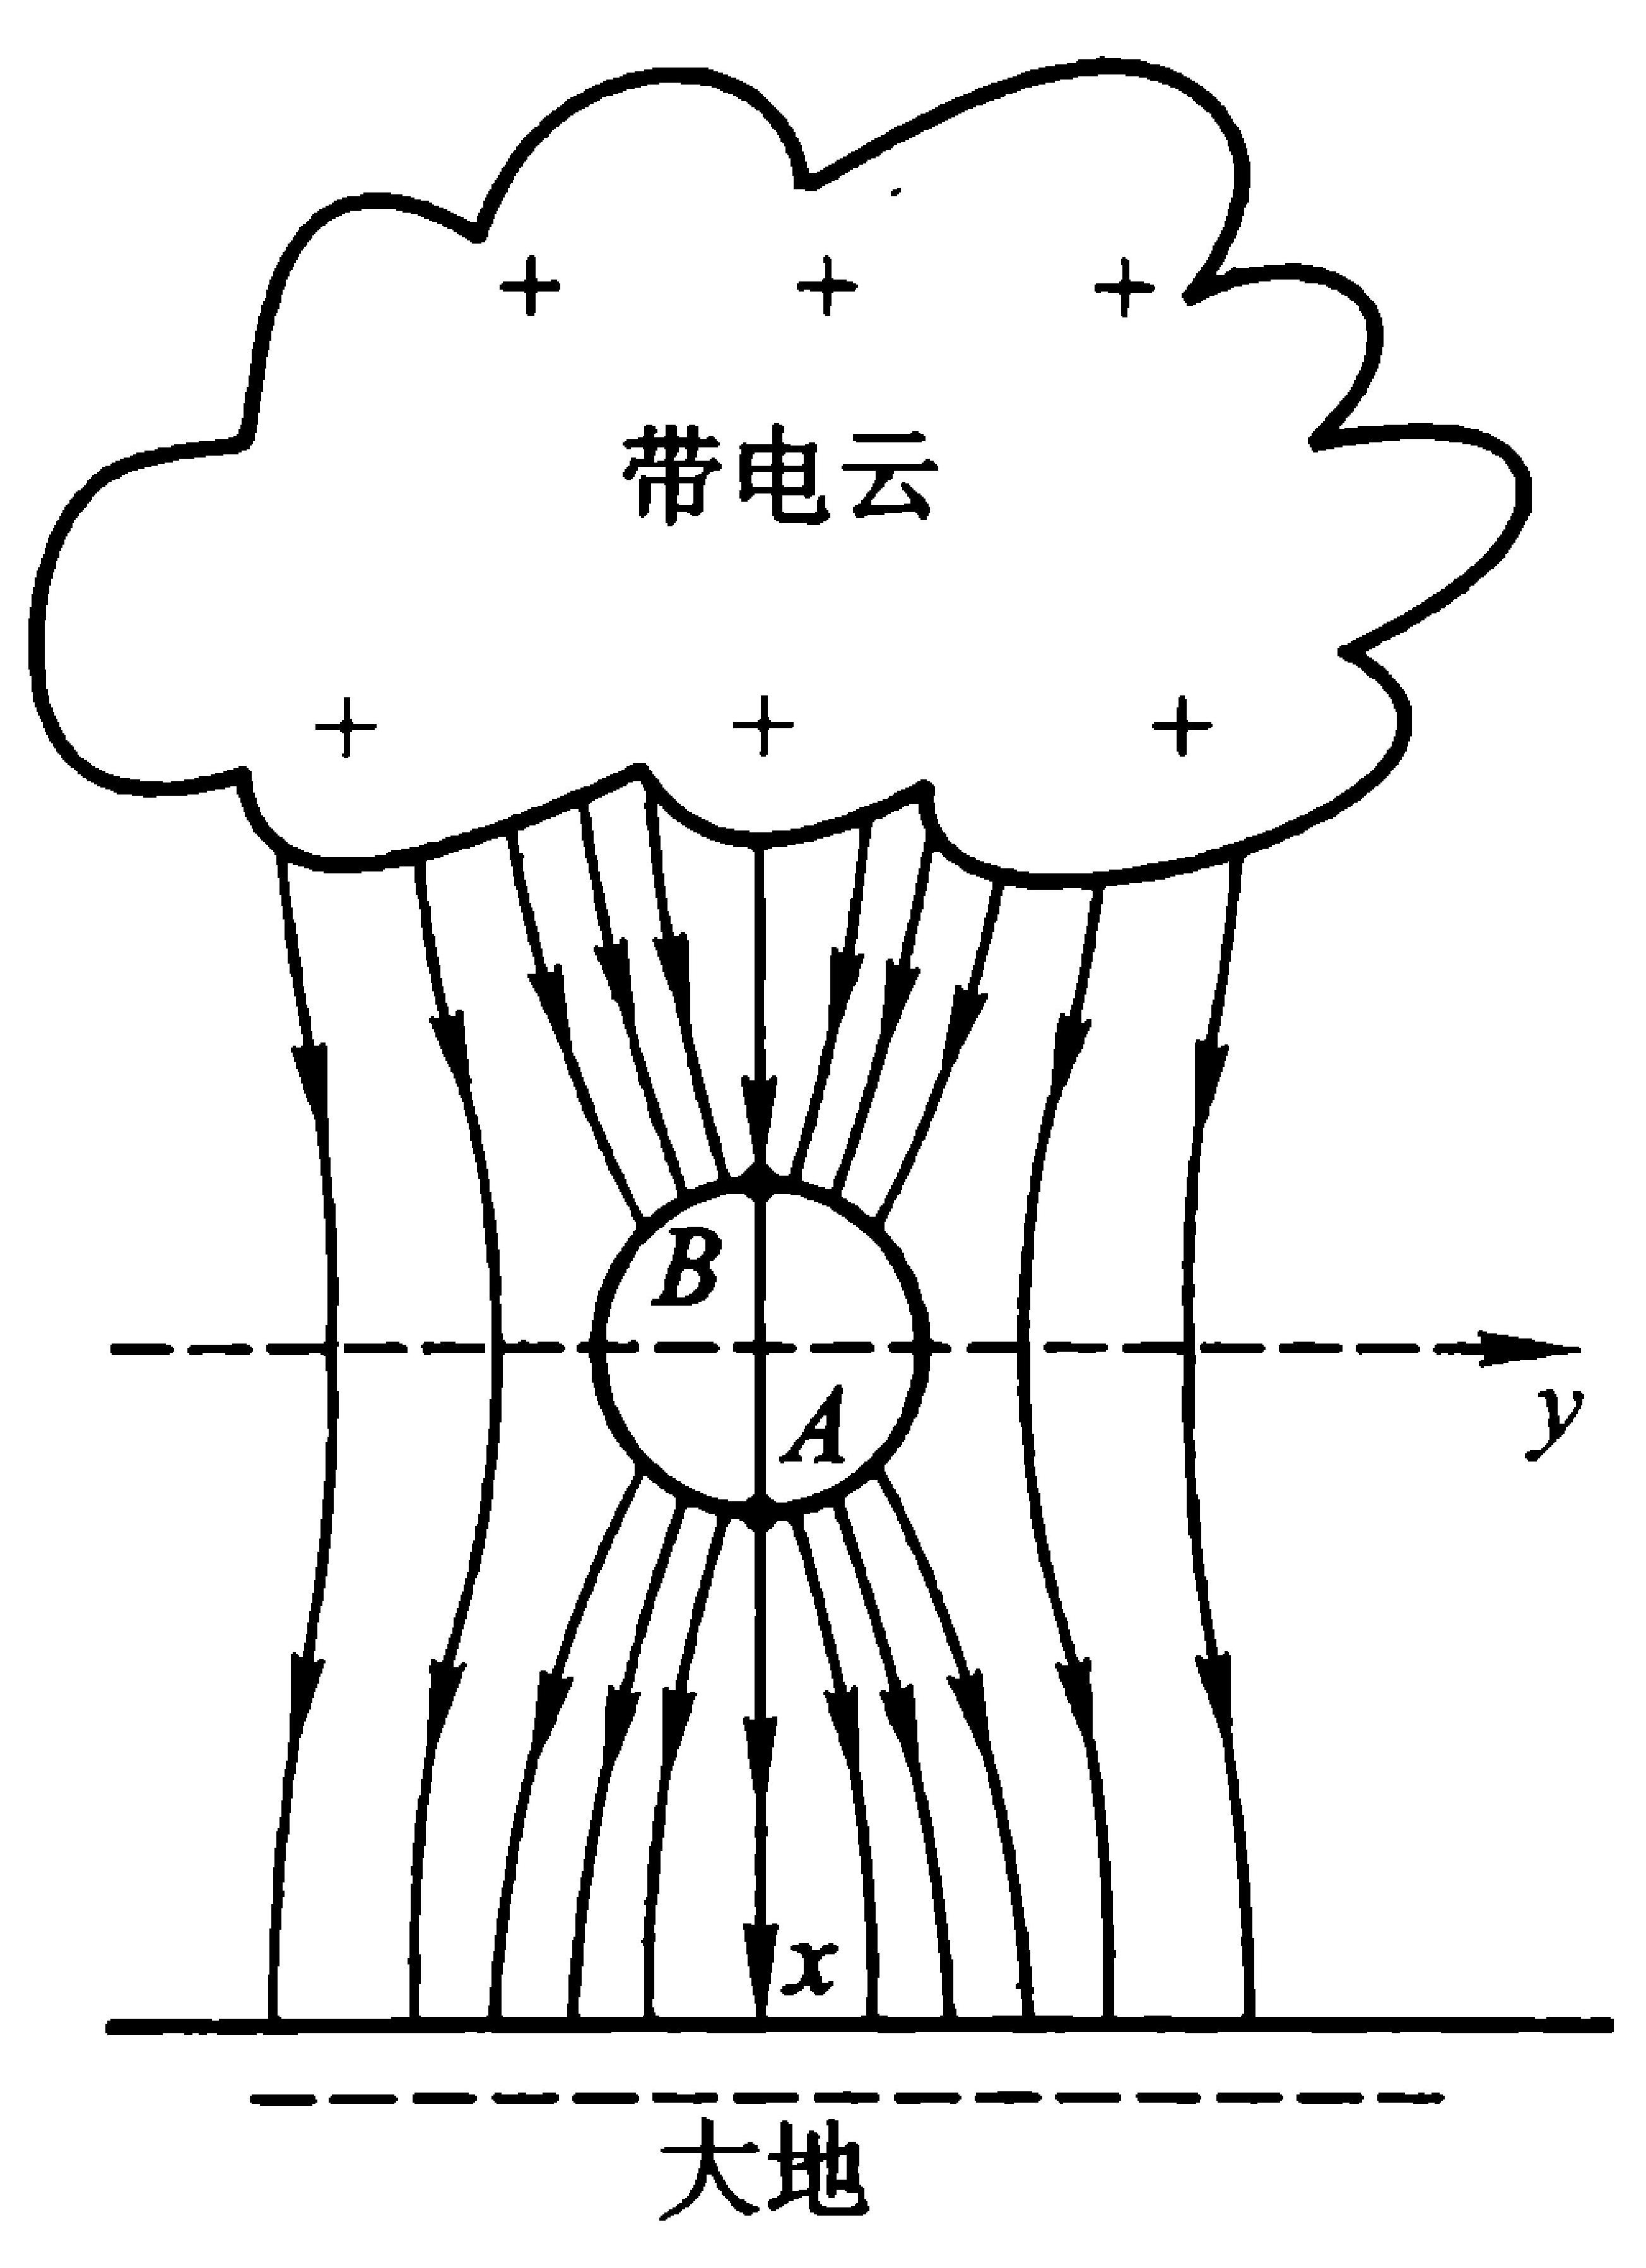
\includegraphics[height=0.72\textheight]{../../lecture/mathphyequations/wire.jpg}
    \end{column}
  \end{columns}
\end{frame}

\begin{frame}{圆上不能把 $X$ 和 $Y$ 分开}
  导体外面没有电荷，势满足 $V_{xx}+V_{yy}=0$。边界是圆 $x^2+y^2=a^2$。若仍设 $V=X(x)Y(y)$，边界上
  \begin{equation*}
    X(x)\,Y\bigl(\sqrt{a^2-x^2}\bigr)=0,
  \end{equation*}
  $X$ 和 $Y$ 缠在一起，分不出各自的条件。
  \vspace{0.4em}
  换到极坐标，这条边界就是 $r=a$，一个变量被固定住了。
\end{frame}

\begin{frame}{极坐标中的拉普拉斯方程}
  在 $r>a$，
  \begin{equation*}
    V_{rr}+\frac{1}{r}V_r+\frac{1}{r^2}V_{\phi\phi}=0.
  \end{equation*}
  导体是等势体，我们把这个等势取成零，于是 $V(a,\phi)=0$。有物理意义的是势差。
  \vspace{0.3em}
  $x$ 轴取得和背景场 $\mathbf{E}_0$ 平行。
\end{frame}

\begin{frame}{远场}
  远处 $E_x=E_0$，$E_y=0$，所以 $-\partial V/\partial x=E_0$。均匀场的势是 $-E_0 x=-E_0 r\cos\phi$。
  \vspace{0.3em}
  圆柱每单位长度还带电 $q_0$，远处多一项 $-(q_0/(2\pi\varepsilon_0))\ln r$。合起来
  \begin{equation*}
    V(r,\phi)\sim
    V_{\infty}-\frac{q_0}{2\pi\varepsilon_0}\ln r-E_0 r\cos\phi
    \qquad (r\to\infty).
  \end{equation*}
  常数 $V_{\infty}$ 随势的零点一起走。导体已经取成零势，这个常数会由 $r=a$ 上的条件定下来。
\end{frame}

\subsection{分离变量}

\begin{frame}{角向与径向分开}
  设 $V=R(r)\Phi(\phi)$。代进拉普拉斯方程，除以 $R\Phi$，再乘 $r^2$，
  \begin{equation*}
    \frac{r}{R}\frac{\mathrm{d}}{\mathrm{d}r}
      \left(r\frac{\mathrm{d}R}{\mathrm{d}r}\right)
    =-\frac{\Phi''}{\Phi}=m^2.
  \end{equation*}
  左边只含 $r$，右边只含 $\phi$，两边等于同一个常数。我们把它写成 $m^2$。
\end{frame}

\begin{frame}{周期性选出整数 $m$}
  $\phi$ 增加 $2\pi$ 回到同一个点，所以 $\Phi(\phi+2\pi)=\Phi(\phi)$。于是
  \begin{equation*}
    \Phi''+m^2\Phi=0.
  \end{equation*}
  指数解转一圈回不到原来的值。留下来的是 $\cos(m\phi)$ 和 $\sin(m\phi)$，$m=0,1,2,\ldots$。
  \vspace{0.3em}
  $m$ 因此是整数。这和固定端把 $\lambda$ 收成一串离散值是同一件事：单值性代替了端点条件。
\end{frame}

\begin{frame}{径向欧拉方程}
  径向部分是
  \begin{equation*}
    r^2 R''+r R'-m^2 R=0.
  \end{equation*}
  这是欧拉方程。令 $r=e^{s}$，也就是 $s=\ln r$，则
  \begin{equation*}
    r R_r=R_s,
    \qquad
    r^2 R_{rr}=R_{ss}-R_s.
  \end{equation*}
  代回去得到 $R_{ss}-m^2 R=0$。
\end{frame}

\begin{frame}{径向解}
  $m\geq 1$ 时 $R_{ss}=m^2 R$，
  \begin{equation*}
    R=A e^{ms}+C e^{-ms}=A r^{m}+C r^{-m}.
  \end{equation*}
  $m=0$ 时 $R_{ss}=0$，
  \begin{equation*}
    R=C_0+D_0 s=C_0+D_0\ln r.
  \end{equation*}
  $r^{m}$ 在远处越来越大，$r^{-m}$ 在远处趋于零。圆柱外面的势两种都先写上，等远场来决定哪一些系数为零。
\end{frame}

\begin{frame}{外部调和函数的一般形式}
  \begin{equation*}
    \begin{aligned}
    V={}&C_0+D_0\ln r\\
    &+\sum_{m=1}^{\infty}\Big[
      \bigl(A_m r^{m}+C_m r^{-m}\bigr)\cos(m\phi)\\
      &\qquad
      +\bigl(B_m r^{m}+D_m r^{-m}\bigr)\sin(m\phi)
    \Big].
    \end{aligned}
  \end{equation*}
  若是圆内的问题，$\ln r$ 和 $r^{-m}$ 在原点发散，应当丢掉。这里区域是 $r>a$，原点不在里面，这两项可以留。
\end{frame}

\subsection{两边的边界条件}

\begin{frame}{导体表面}
  $V(a,\phi)=0$ 对每个 $\phi$ 都成立。傅里叶系数唯一，所以每一项的径向系数在 $r=a$ 上为零：
  \begin{equation*}
    C_0+D_0\ln a=0,
    \qquad
    A_m a^{m}+C_m a^{-m}=0,
    \qquad
    B_m a^{m}+D_m a^{-m}=0.
  \end{equation*}
  即
  \begin{equation*}
    C_0=-D_0\ln a,
    \qquad
    C_m=-a^{2m}A_m,
    \qquad
    D_m=-a^{2m}B_m.
  \end{equation*}
  增长的 $r^{m}$ 都配上一个衰减的 $r^{-m}$，两者在柱面上抵消。
\end{frame}

\begin{frame}{远场丢掉 $m>1$}
  远处给的势最高只到 $r$ 的一次。$m>1$ 的 $r^{m}$ 比这还高，系数必须为零，远场才对得上。
  \begin{itemize}
    \item $m\geq 2$：$A_m=B_m=0$，于是 $C_m=D_m=0$。
    \item 远场里没有 $\sin\phi$，所以 $m=1$ 的正弦系数 $B_1=D_1=0$。
    \item 余弦这一项要配上 $-E_0 r\cos\phi$，因此 $A_1=-E_0$，再由柱面条件 $C_1=E_0 a^2$。
  \end{itemize}
\end{frame}

\begin{frame}{对数项}
  远场里 $\ln r$ 的系数给出 $D_0=-q_0/(2\pi\varepsilon_0)$。柱面上 $C_0=-D_0\ln a$，所以
  \begin{equation*}
    C_0+D_0\ln r
    =D_0\ln\frac{r}{a}
    =\frac{q_0}{2\pi\varepsilon_0}\ln\frac{a}{r}.
  \end{equation*}
  $V_{\infty}$ 已经放进导体零势的选择里，式子里不再单写。
\end{frame}

\begin{frame}{中性圆柱}
  $q_0=0$ 时对数项消失，只留下 $m=1$ 的余弦：
  \begin{equation*}
    \boxed{V(r,\phi)
    =-E_0\left(r-\frac{a^2}{r}\right)\cos\phi.}
  \end{equation*}
  $-E_0 r\cos\phi$ 是原来的均匀场，$E_0(a^2/r)\cos\phi$ 是感应电荷带来的修正。两项在 $r=a$ 上相加为零，导体保持零势。
\end{frame}

\begin{frame}{代回边界和远场}
  把这个势放回 $r=a$：
  \begin{equation*}
    r-\frac{a^2}{r}=a-a=0,
  \end{equation*}
  所以 $V(a,\phi)=0$，和导体零势一致。
  \vspace{0.35em}
  $r\to\infty$ 时 $a^2/r\to 0$，$V\sim -E_0 r\cos\phi=-E_0 x$，于是
  \begin{equation*}
    E_x=-\frac{\partial V}{\partial x}\to E_0,
    \qquad E_y\to 0.
  \end{equation*}
  柱子附近的场被扭曲了；走远以后，电场回到原来的均匀场。方程、柱面和远场这三处都核对过了。
\end{frame}

\begin{frame}{带电圆柱}
  每单位长度带电 $q_0$ 时，再加上对数项：
  \begin{equation*}
    V(r,\phi)
    =\frac{q_0}{2\pi\varepsilon_0}\ln\frac{a}{r}
    -E_0\left(r-\frac{a^2}{r}\right)\cos\phi.
  \end{equation*}
  这一项就是长直圆柱上电荷的势。在圆柱外面，它和放在轴上的线电荷写成同一个形式。
  \vspace{0.3em}
  均匀场和感应电荷的那一对仍和中性时一样。对数项不随 $\phi$ 变化，柱面上的余弦搭配保持不变。
\end{frame}

\begin{frame}{表面场增强到 $2E_0$}
  \begin{columns}[c]
    \begin{column}{0.54\textwidth}
      对中性圆柱，
      \begin{align*}
        E_r&=-\frac{\partial V}{\partial r}\\
        &=E_0\Bigl(1+\frac{a^2}{r^2}\Bigr)\cos\phi.
      \end{align*}
      在 $r=a$ 上，$E_r=2E_0\cos\phi$。$\phi=0$ 和 $\phi=\pi$ 两点，法向场的大小都是 $2E_0$。
      \vspace{0.35em}
      外场指向的两端，表面场被加强，电击穿也更容易从这里开始。
    \end{column}
    \begin{column}{0.44\textwidth}
      \centering
      \scalebox{0.78}{\begin{tikzpicture}[font=\small, >=Stealth,
    vec/.style={-{Stealth[length=2mm]}, line width=0.7pt}]
  \draw[gray!35, thin] (-2.6,0) -- (2.6,0) node[right] {$x$};
  \draw[gray!35, thin] (0,-1.9) -- (0,1.9) node[above] {$y$};
  \fill[blue!8] (0,0) circle (0.85);
  \draw[blue!70!black, thick] (0,0) circle (0.85);
  \node at (0,0) {导体};
  \foreach \y in {-1.35,-0.45,0.45,1.35} {
    \draw[vec, gray!80] (-2.45,\y) -- (-1.15,\y);
    \draw[vec, gray!80] (1.15,\y) -- (2.45,\y);
  }
  \draw[vec, red!70!black] (0.85,0) -- (1.55,0) node[midway, above] {$2E_0$};
  \draw[vec, red!70!black] (-1.55,0) -- (-0.85,0);
  \node[font=\scriptsize, gray] at (2.05,1.55) {$\mathbf{E}_0$};
  \node[font=\scriptsize] at (0,-1.55) {$r=a$};
\end{tikzpicture}
}
    \end{column}
  \end{columns}
\end{frame}

\begin{frame}{赤道上势等于导体}
  在 $y$ 轴上，$\phi=\pm\pi/2$，$\cos\phi=0$。均匀场和感应修正的势都是零。
  \vspace{0.3em}
  中性圆柱在这两条射线上的势等于导体的势。若圆柱带电，赤道上只留下对数项，也就是线电荷的势。
\end{frame}

\begin{frame}{这个例子说明什么}
  回头看这个例子，坐标是顺着边界选的。
  圆边界在极坐标里变成 $r=a$。角向转一圈必须回到原处，$m$ 因此取整数。柱面把 $r^{m}$ 和 $r^{-m}$ 配成对，远场再决定留下哪些项。
  \vspace{0.35em}
  步骤和固定弦相同：分离变量，求本征值，叠加，最后用边界和远场定系数。
\end{frame}

% % =============================================================
% \section{全章小结}

% \begin{frame}{三条方程与三类问题}
%   \begin{align*}
%     u_{tt}-a^2\nabla^2 u&=f
%       && \text{双曲：有限速度传播},\\
%     u_t-\kappa\nabla^2 u&=f
%       && \text{抛物：扩散抹平},\\
%     \nabla^2 u&=f
%       && \text{椭圆：平衡或势}.
%   \end{align*}
%   两个自变量时，类型由 $\Delta=B^2-AC$ 的符号决定。非奇异的坐标变换不改变这个符号。
% \end{frame}

% \begin{frame}{定解与求解}
%   狄利克雷指定场本身，诺伊曼指定法向通量，罗宾把二者线性组合。
%   \vspace{0.4em}
%   齐次线性问题可以叠加。分离变量把边界条件变成本征值问题，初始数据或另一侧边界再来定系数。
%   固定弦的系数是正弦级数；圆柱外的势是 $\ln r$、$r^{\pm m}$ 乘上三角函数。
% \end{frame}

% \begin{frame}{两条用了整章的公式}
%   两端固定的弦：
%   \begin{equation*}
%     u(x,t)=\sum_{n=1}^{\infty}
%     \bigl[A_n\cos(\omega_n t)+B_n\sin(\omega_n t)\bigr]
%     \sin\Bigl(\frac{n\pi x}{\ell}\Bigr),
%     \quad \omega_n=\frac{n\pi a}{\ell}.
%   \end{equation*}
%   均匀电场中的中性导体圆柱：
%   \begin{equation*}
%     V(r,\phi)=-E_0\left(r-\frac{a^2}{r}\right)\cos\phi.
%   \end{equation*}
% \end{frame}

% \begin{frame}{延伸阅读}
%   \begin{itemize}
%     \item Strauss, \textit{Partial Differential Equations}.
%     \item Tikhonov \& Samarskii, \textit{Equations of Mathematical Physics}.
%     \item Courant \& Hilbert, \textit{Methods of Mathematical Physics}, Vol.~II.
%   \end{itemize}
%   \vspace{0.6em}
%   傅里叶级数本身、球坐标和柱坐标里的特殊函数，以及格林函数，分别在后面的章节展开。
% \end{frame}

\end{document}
